\chapter{Introduction}

We wish to spend our time more productively, but we sink hours into social media; we wish to learn new languages, but we get too busy to practice; we wish to be more healthy, but we do not maintain our exercise routines~\cite{consolvo2009theory}. Inspired by situations like these, \textit{behavior change} systems help people build new habits and retain them~\cite{consolvo2008activity,froehlich2009ubigreen,kay2012lullaby,kim2016timeaware}. Behavior change systems draw on theories of persuasion and influence~\cite{fogg2002persuasive,cialdini1987influence} to introduce \textit{interventions}: interaction designs that variously inform, nudge, and encourage people to engage in behaviors more in line with their goals.

There are large numbers of users who wish to achieve behavior change goals, and a large design space for interventions. Thus, there is a natural opportunity to explore the design space of interventions and find what interventions works best, by testing them out with users. However, the existing ecosystem of behavior change tools does not make full use of this resource.

Behavior change tools, both those tailored towards commercial mass-market adoption by end users as well as research systems, have tended to employ a one-size-fits-all approach, implementing only a single behavior change intervention and giving the same experience to all users. Users can choose and select between different behavior change apps and extensions to find what they believe works well for them. However, because different apps are developed by different companies which do not share data, they cannot compare the interventions. They thus miss out on a rich opportunity for improving the behavior change systems via experimentation.
% \msb{we're not necessarily competing here against mass market tools, we're showing that we're pushing forward the state of the art. is this generally true of most systems, not just mass market ones?} \geza{done}

Research studies on behavior change, in contrast, have tended to compare only a small number of interventions, with small numbers of paid participants. They thus miss out on the ecological validity, scale, and statistical power that systems targeting the mass market of end users can enjoy.

Our key insight was that we can find an alignment the goals of behavior change researchers and end users, by building a behavior change tool targeted towards the mass market that also runs useful experiments. End users benefit by being able to use a high-quality behavior change tool where the design choices are experimentally tested and validated. Researchers benefit by being able to run ecologically valid behavior change experiments at scale.

While we believe that many domains can potentially benefit from in-the-wild behavior change experimentation, we believe that online behavior change is particularly well-suited. As interventions can be distributed as software that requires only a click to install, this enables us to recruit a wide range of participants worldwide for free. Additionally, as our computers and phones can display arbitrary interactive content, this paradigm allows us to experiment with a limitless number of different interventions, and change interventions at any time. Finally, as device usage can be precisely monitored down to the level of which webpage or app was open each second, we can easily measure the effectiveness of interventions and adapt them accordingly.

As a result, we built HabitLab, an in-the-wild experimentation platform for helping users reduce their time online and on their phones. HabitLab is implemented as both a Chrome extension and an Android app, and is currently used by over 12,000 daily active users. Users select sites and apps they wish to spend less time on, and HabitLab deploys a variety of interventions to help them achieve their goals. The platform enables us to run a number of A/B tests comparing interventions and aspects of behavior change systems.

% In addition to the HabitLab platform itself, this thesis also presents three sets of studies we ran with it.

\begin{figure}
  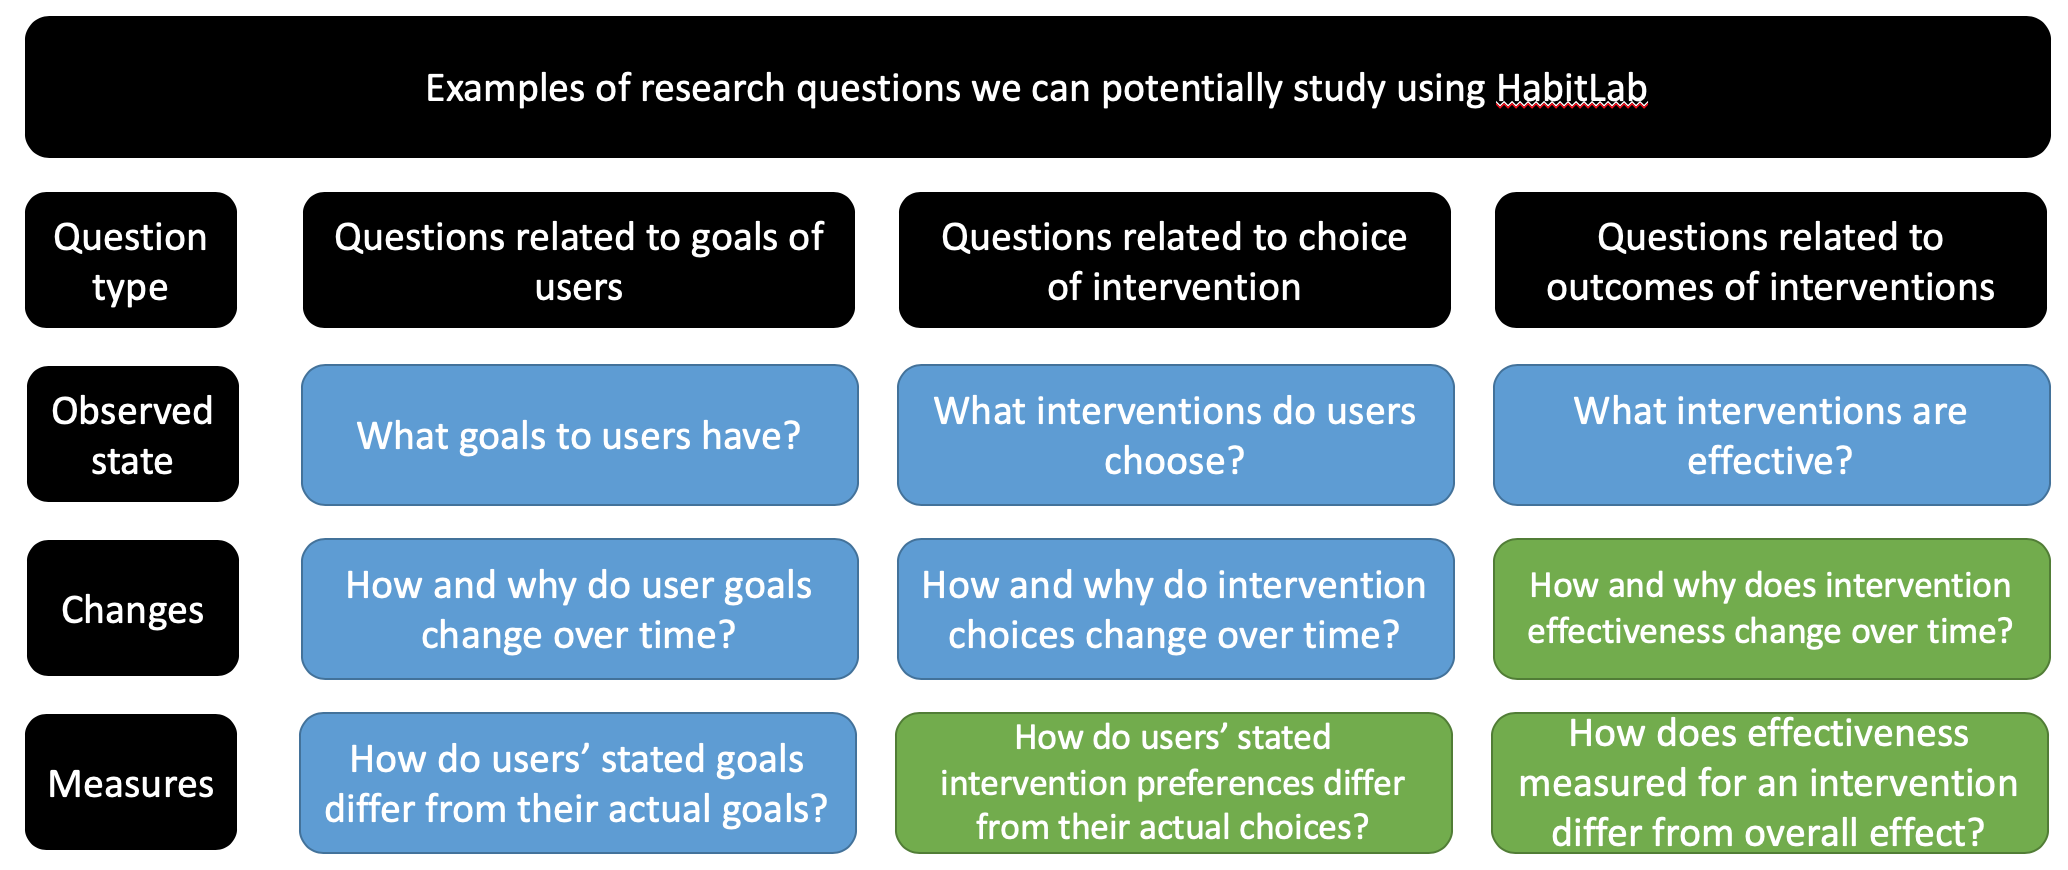
\includegraphics[width=\linewidth]{figuresI/researchquestions.png}
  \caption{Examples of research questions that can be studied with the HabitLab system and the general space of questions they occupy. Research questions we study in this thesis are shown in green.}
  \label{fig:researchquestions}
\end{figure}


There is a rich set of studies we can run with a tool such as HabitLab. The general paradigm is that users specify goals, interventions are deployed to help them achieve those goals, and we measure the outcomes of the interventions. At a high level, we can thus categorize the space of possible research studies that a platform such as HabitLab can conduct as below. A more detailed classification is shown in Figure~\ref{fig:researchquestions}.

\begin{enumerate}
\item Studies analyzing users' goals
\item Studies analyzing the choice of interventions to help users achieve those goals
\item Studies analyzing the outcomes of interventions
\end{enumerate}

We believe that the HabitLab system is uniquely well-suited for investigating the letter two classes of problems within behavior change. Specifically, it allows us to quickly test a variety of different choices of interventions -- as we can make arbitrary changes to websites, or show arbitrary overlays over the phone screen. Additionally, it also enables us to precisely measure the outcomes of the interventions -- specifically, we can directly observe the amount of time users spend on sites.

In addition to demonstrating the technical feasibility of such an in-the-wild experimentation system by building it and using it for studies, we demonstrate via HabitLab's large install base that it is possible to align user incentives with those of researchers within this behavior change domain. Many other studies rely on having to pay or force participants to use the system, as the primary beneficiary of the research is the researcher -- but with HabitLab, users benefit from the research, as the insights we gain from user behavior data allows the system to better help users achieve their goals.

%\msb{summarize what we learn on the design and systems side. that we demonstrate that it's possible to ...} \geza{done}

\section{Thesis Overview}

In this thesis we will first present the HabitLab system. Then we will describe a pair of studies conducted on the HabitLab system, which both study secondary effects that influence the intervention outcomes that we observe. %Then we will present three studies conducted on the HabitLab system: two analyzing the outcomes of interventions, and one study analyzing the choice of interventions to help users achieve those goals.

%\msb{typically we use \\ref and \\label to actually number the chapters here} \geza{done}

\subsubsection{Chapter~\ref{ch:system}: The HabitLab System}

We first describe the HabitLab system itself, the design process, the interventions, how we were able to amass a userbase of 12,000 daily active users via an in-the-wild deployment, and the demographics of those users.

\subsubsection{Chapter~\ref{ch:rotation}: Intervention Rotation Study}

The first study we present asks whether the effectiveness of interventions decline over time. Prior literature suggests this is a possibility, as engagement-boosting novelty effects have been attested in numerous domains. We find that an intervention that is repeatedly presented does indeed decline in effectiveness over time, and that a strategy of rotating between different interventions helps boost effectiveness. This boost comes at the cost of increased attrition, which we find mostly to be due to incorrect mental models, as users are unaccustomed to interventions changing. A simple design helping explain the intervention rotation to users and give them a sense of control significantly reduces this resulting attrition.

\subsubsection{Chapter~\ref{ch:conservation}: Time Redistribution Study}

The second study concerns itself with whether intervention outcomes are actually what we expect them to be looking at just the time spent on the targeted site or app. Prior literature suggests that willpower is limited, hence we may expect that reducing time on one app, site, or device may increase time spent on others. Other literature suggests that procrastination begets more procrastination by trapping us into a habit loop, hence we may expect that reducing time on one app, site, or device may reduce time spent on others. We find that in the case of site usage on browsers, reducing time on one site results in a reduction of time spent on others. In the case of app usage on mobile, we observe that reducing time on one app does not affect time on others. Likewise, in the case of devices, reducing time on one device does not affect time on others.

% The third study is about how users' preferences 

\section{Contributions}

The contributions of this thesis are:

\begin{enumerate}
\item HabitLab, a system for conducting in-the wild behavior change experiments online. It has been widely adopted with a 12,000 user install base across the browser and mobile platforms, showing that in-the-wild behavior change systems can be used to conduct large-scale experiments.
\item A set of design principles we have developed for in-the-wild experimentation platforms, which help researchers navigate conflicts that may emerge between the needs of end users and the scientific needs of researchers.
\item A set of studies conducted on HabitLab showing that static interventions decline in effectiveness over time, and that rotating interventions can improve their effectiveness.
\item A set of studies conducted on HabitLab showing that interventions can sometimes have beneficial secondary effects, reducing time spent on non-targeted sites.
\end{enumerate}

%\msb{between 1 and 2, I'd like to see articulation of what the generalizable ideas are from the design of HabitLab. The contribution here isn't just HabitLab, it's the design ideas that HabitLab embodies.} \geza{done}

% our contributions in this thesis are

These studies show that our paradigm of in-the-wild experimentation, as realized in the domain of online behavior change via the HabitLab, can work to find novel insights about behavior change systems. We hope this work can help designers build better systems for online behavior change, and promote analogous in-the-wild experimentation in other behavior change domains.



